\section{Current Results and Projections}
\subsection{Current Results}
Peculiar velocity surveys have already been  used to measure
the effective $fD$ in redshift bins  (referred to as $f\sigma_8$), though not to a level where  gravity models can be precisely distinguished.
 \citet{2017MNRAS.471..839A} use 6dFGS peculiar velocities using  Fundamental Plane distances of elliptical galaxies to estimate absolute magnitudes
 with
 $\sim 0.43$~mag  precision, yielding a 15\% uncertainty in $fD$ at $z\approx 0$.
The upcoming 
TAIPAN survey \citep{2017PASA...34...47D} will obtain Fundamental Plane galaxies with densities of $n_g \sim 10^{-3}h^3$\,Mpc$^{-3}$,
and the WALLABY+WNSHS surveys \citep{2008ExA....22..151J} will obtain Tully-Fisher distances (based on the $\sim 0.48$~mag calibration of absolute magnitude based on the  HI 21cm line width)
of galaxies with densities $n_g \sim 2\times 10^{-2} - 10^{-4} h^3$\,Mpc$^{-3}$ from
$z=0-0.1$ covering 75\% of the sky.
These surveys combined are projected to have 3\% uncertainties in $fD$ \citep{2017MNRAS.464.2517H}.
For reference, DESI projects a 10\% precision of $fD$ at $z \approx 0.3$  by looking 
for signatures (Redshift Space Distortions; RSD) expected from galaxies infalling toward mass overdensities.
Relative to galaxies with  Fundamental Plane or Tully-Fisher distances, 
SN~Ia host galaxies currently have significantly lower number density but have better per-object peculiar velocity precision.
Existing SN~Ia samples
have been used to test and ultimately find spatial correlations in peculiar velocities that may be attributed to the growth of structure
\citep{PhysRevLett.99.081301,2008MNRAS.389L..47A,2014MNRAS.444.3926J,2015JCAP...12..033H, 2017JCAP...05..015H}.
SNe~Ia discovered by ASAS-SN, ATLAS, and ZTF \citep{2014ApJ...788...48S,2018PASP..130f4505T,2019PASP..131a8002B} over the next several years will provide first probative measures of $fD$ at $z<0.1$.
%Measurement of the velocity field using LSST-discovered
%SNe~Ia has been quantified by \citep{2011PhRvD..83d3004B,2017JCAP...01..060O}

\subsection{Projections}
Two advances in the upcoming decade will make SN~Ia peculiar velocities more powerful.
First, the precision of SN~Ia distances can be improved.  The commonly-used empirical 2-parameter spectral model yields  absolute magnitude
dispersion $\sigma_M \gtrsim 0.12$~mag.  However, SNe transmit more information than just the light-curve shape and single color used in current SN models.
Recent studies indicate that with the right data, SN absolute
magnitudes can be calibrated to $\sigma_M \lesssim 0.08$ mag \citep[see e.g.][]{2012MNRAS.425.1007B, 2015ApJ...815...58F}. 
Though not yet
established, it is anticipated that such a reduction in intrinsic dispersion comes with a reduction in the magnitude bias correlated with host-galaxy properties
that is observed using current calibrations.  At this precision the intrinsic velocity dispersion  at $z=0.028$ is  $300$~km\,s$^{-1}$, i.e.\ a single SN~Ia  is of such quality as to
measure a peculiar velocity with $S/N \sim 1$.
 If corrections of all SNe~Ia are not possible, the use of SN~Ia subclasses is an option though at the expense of reducing the
numbers of velocity probes.
Secondly,  in the upcoming decade cadenced wide-field imaging surveys such as ZTF2 and LSST
  will increase the number of identified  $z<0.2$ Type~Ia supernovae from the hundreds to the
hundreds of thousands; over the course of 10-years, LSST will find $\sim150,000$ $z<0.2$ SNe~Ia
 for which good light curves can be measured, corresponding to a  number density of $n \sim 5\times 10^{-4}h^3$\,Mpc$^{-3}$.
  This sample has comparable
 number density and more galaxies at deeper redshifts than projected by WALLABY and TAIPAN.  With similar densities,
 the (two) ten-year SN~Ia survey will have
 a (6) 29$\times$ reduction in shot-noise, $\sigma^2_M/n$, relative to the Fundamental Plane survey of TAIPAN.

A SN~Ia peculiar velocity program hinges on  SN discoveries, the number density $n$ of which
depends on the cadenced wide-field imaging survey used for the search.    
It is thus convenient to make projections for upcoming programs
based on the imaging survey; the projections here use ZTF2 and LSST 
as canonical representatives.
Keep in mind that other follow-up resources determine the distance precision $\sigma_M$, the other important parameter
that affects projections.


The primary sources of systematic error in a high-redshift supernova Hubble diagram are not as important for a low-redshift
peculiar velocity survey.  A Hubble diagram that spans a broad redshift range requires absolute color calibration over the corresponding observer-frame
wavelength range and control over the different populations over the span of cosmic time from which SNe are drawn.  High-redshift peculiar
velocity measurements do not have much sensitivity to $\gamma$, and a SN survey confined to lower redshifts is less sensitive to
color-calibration uncertainties and population evolution.

Details on the assumptions made for the calculations that follow can be found in \citet{2019BAAS...51c.140K}.

\subsubsection{Near-Term: ZTF2}
ZTF2 and TAIPAN are near-term surveys that will measure peculiar velocities, the former using SNe~Ia and the latter
using Fundamental Plane Galaxies.  Both have roughly
 $z_{\text{max}}=0.09$ and $\Omega = 2\pi$.
Uncertainties in $\gamma$ for surveys with this depth and solid-angle coverage 
are shown as a function of number of sources $N$ and $\sigma_M$ in Figure~\ref{surface:fig}. 

The positions of ZTF2 and TAIPAN are marked
in the figure, with the former showing both  a conservative $\sigma_M=0.12$~mag and aggressive $\sigma_M=0.08$~mag.
The former is the uncertainty that could be achieved with ZTF2 photometry alone, the latter with additional
SN follow-up.
ZTF2 and TAIPAN lie in opposite ends of the figure, there are small numbers of ZTF2 SNe with precise distances
whereas there are many TAIPAN Fundamental Plane galaxies with imprecise distances. 
Conservative ZTF2 and TAIPAN
are projected to give similar precisions $\sigma_ \gamma = 0.060$, whereas  aggressive ZTF2 gives a more constraining
$\sigma_ \gamma = 0.048$.  
Recall that the difference in $\gamma$  between GR and the $f(R)$ and DGP gravity is 0.13, meaning that the surveys
can already distinguish between these models to $2-3 \sigma$.

\begin{figure}
\centering
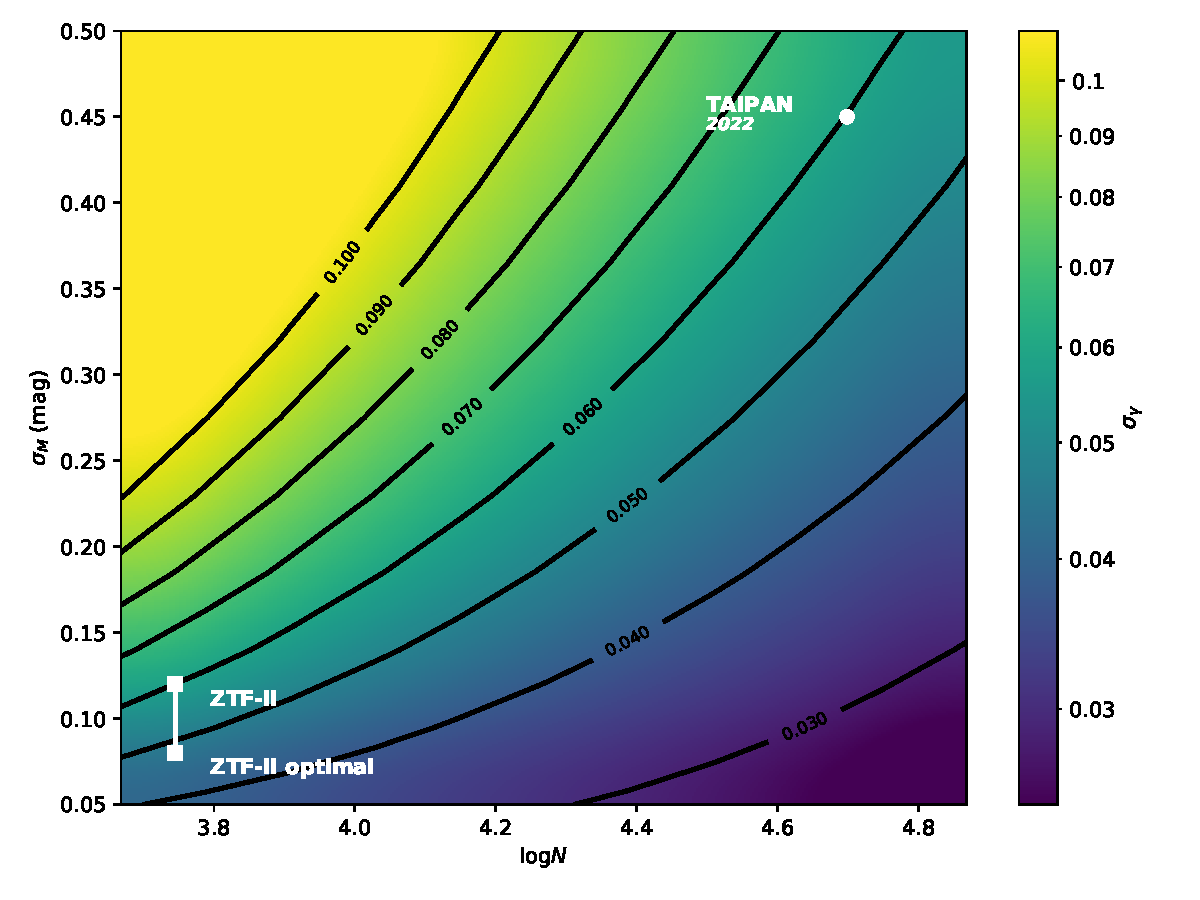
\includegraphics[width=0.6\textwidth]{src/surface1.pdf}
\caption{Uncertainties in $\gamma$ for surveys  with $z_{\text{max}}=0.09$ and $\Omega = 2\pi$
are shown as a function of number of sources $N$ and $\sigma_M$.  The positions of ZTF2 and TAIPAN are marked,
with the former showing both  a conservative $\sigma_M=0.12$~mag and an aggressive $\sigma_M=0.08$~mag.
\label{surface:fig}}
\end{figure}

An important distinction between the surveys is
that TAIPAN will observe almost all available Fundamental Plane galaxies in the local volume, meaning that no additional observing can
increase the number density $n$ and decrease $\sigma_\gamma$.  On the other hand, the number density of supernova increases
linearly with time, there is continued room for decreased $\sigma_\gamma$ with longer surveys  as ZTF2 is not  sample-variance limited 


ZTF2 and TAIPAN are not in competition but are complementary.  Being in different hemispheres, the two surveys
cover different parts of sky, meaning that their two independent results can be
combined  quadratically to produce a reduced joint uncertainty. 

\subsubsection{Long-Term: LSST}
A long-term supernova peculiar-velocity survey can be performed with SNe~Ia discovered by LSST.
As a 10-year survey, LSST generates higher supernova number densities to fainter limiting magnitude than  ZTF2,
making possible significantly improved constraints on the growth index.
All the proposed LSST surveys have complete SN~Ia discovery out to $z=0.3$.
The expected distance uncertainties derived from LSST light curves vary greatly depending on observing strategy, but at best
is expected to be $\sigma_M=0.12$~mag. Some strategies provide SN discovery but much poorer light curves
and distances.   As with the ZTF2 survey,  lower magnitude uncertainties
can be achieved with supplemental data.

Uncertainties in $\gamma$ for surveys with a 10-year duration   and $\Omega=2\pi$ sky coverage, applicable to the LSST WFD survey, 
are shown as a function of limiting  redshift $z_{max}$ and $\sigma_M$ in Figure~\ref{lsst:fig}.
The redshift depth afforded by LSST provides significant improvement relative to the shallower ZTF2 survey.
After 10 years, the region with $z_{max}<0.1$ has $\sigma_\gamma$ that is only weakly $\sigma_M$-dependent, 
which reflects the relatively strong sample variance in the small local survey volume.  
As $\sigma_\gamma$ quickly increases for surveys shallower than the $z_{\text{max}}=0.09$ 
of ZTF2,
better growth index constraints
are achieved by going to $z_{max}>0.1$.
The gradient in decreasing $\sigma_\gamma$ does shallow out with increasing redshift despite the increased survey volume, 
as the velocity uncertainties degrade with redshift for a fixed $\sigma_M$.

\begin{figure}
\centering
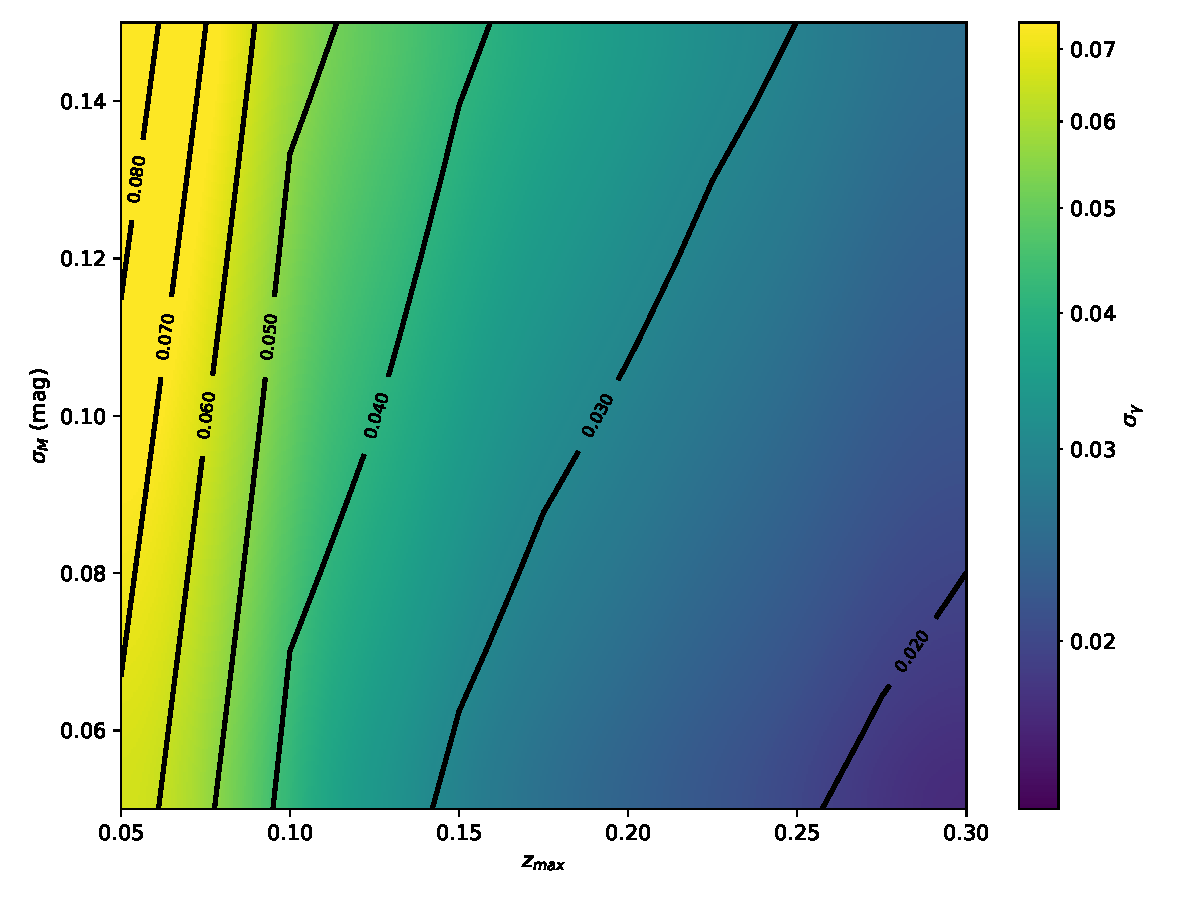
\includegraphics[width=0.6\textwidth]{src/surface2.pdf}
\caption{Uncertainties in $\gamma$ for surveys with a 10-year duration and  and $\Omega=2\pi$ sky coverage 
are shown as a function of limiting  redshift $z_{max}$ and $\sigma_M$.
\label{lsst:fig}}
\end{figure}

\subsection{Complementarity with High-$z$ redshift surveys}
Combined low-redshift peculiar velocity and high-redshift RSD $fD$ measurements (i.e.\ from DESI) are highly complementary as together they probe the
$\gamma$-dependent shape of $fD(z)$ (not just its normalization) and potential scale-dependent influence of gravitational models.  
\added[id=2]{The latter is true because 
the $k_{\text{max}}$ of linear modes for the RSD measurement is higher than that of the low-redshift peculiar velocity measurement.}

\section{Plan for a Peculiar Velocity Program}
The projections for measuring $\gamma$ with ZTF2 and LSST SN~Ia discoveries
show the power of peculiar velocities surveys at low redshift.
This  tracer provides an unmatched  new window with which to test gravity and the source of the accelerating expansion of the Universe.
We propose the following course of research for the upcoming decade.

\subsection{Present}
The current goals are to provide a proof of concept of a SN peculiar velocity survey while developing domain
expertise and pipelines that can be used in future experiments.

Kim has developed a SNFactory/ZTF peculiar-velocity analysis framework with a postdoc.  Its distinguishing features is that it is likelihood-based
including both density and peculiar velocities.  The complexity of including fitting the underlying mass density field in the model
is addressed through Hamiltonian Monte Carlo.  Analytic expressions for the partial derivatives of the likelihood are coded,
avoiding the computational limitations of {\it autodiff} in STAN.  A end-to-end implementation is complete, validation of it is ongoing.

The first application o the analysis pipeline will be for SNFactory supernovae.  A next analysis will be of ZTF-discovered 
SNe when those data are ready.  The plan is for a  subset of the required data, precision redshifts of SN host galaxies, to be provided
by DESI.  Additional DESI data contributions are being discussed.

\subsection{Near Term: DESI as TAIPAN-North}

There has been talk of using BGS for a peculiar-velocity survey.  There is some question as to how deep the BGS achieves.  This should be
dug into.

\subsection{Near Term: ZTF2 + DESI}
A near-term peculiar velocity program can already provide the most competitive measurements of $\gamma$ at low redshift.  Engaging in science
now positions LBL for domain leadership in the LSST era.  For its near-term peculiar-velocity program, we advocate a survey using SN~Ia discoveries from ZTF2,
rather than other possible surveys, for the following reasons:
\begin{itemize}
\item A peculiar-velocity survey is already being touted as a primary science driver. As such,
the observing strategy should accommodate our needs.
\item It would be ready to start at the end of ZTF in 2021.
\item It is cheap, with a cost ranging from zero to access public data, to an amount (\$300k?) smaller
than building a new facility.
\item ZTF2 includes SEDMachine for classification of $m<18.5$~mag  transients.
\item It is in the Northern Hemisphere, which complements and is not superseded by LSST. 
Even after the nominal 3-year survey and simultaneous with LSST, the facility remains important for peculiar-velocity studies.
\item It is anticipated that the public plus private collaboration surveys can be designed to generate distance
precisions of $\sigma_M =0.12$~mag, which allow good velocity measurements with SNe~Ia.  (Additional follow-up can lower this uncertainty further.)
\item The limiting redshift $z_{\text{max}} =0.09$ is sufficiently deep  to have a scientifically interesting result $\sigma_\gamma < 0.053$.
There are other SN searches that do not achieve this depth.
\end{itemize}

ZTF2 SN~Ia discoveries are combined with data from other facilities to form a complete PV program.  We propose:
\begin{itemize}
\item DESI will provide the following components of the survey:
\begin{itemize}
\item Discovery Screening -- Provides redshifts for probable host galaxies of new transients, for use in early classification.  A host galaxy may
already have a DESI redshift, may be a BGS target without a redshift but whose observation could be prioritized,  or non-DESI target for which we
make a secondary-target fiber allocation.
\item SN Ia Classification -- Spectroscopy of active transients  through secondary-target fiber allocations within
DESI survey pointings. There
will be $\sim 1$ active $r<21.5$ SN~Ia in every three DESI pointings.  Coordinating DESI pointings such that ``every'' pointing contains
a  ZTF2 discovery can significantly increase the number of classifications, relative to the random (from the transient perspective) default DESI pointings.
Triggered observations of non-DESI pointings is possible, though does not take advantage of DESI multiplexing.
\item Host-galaxy redshift -- Some precise galaxy redshifts may not be available at the end of the ZTF2 survey.  Mopping up of ZTF2 host-galaxy redshifts
can be done efficiently with a single sweep of DESI's MOS.
\end{itemize}
 The $R>2000$ resolution
provides sufficiently precise redshifts so as to make their uncertainties negligible in the $\gamma$ error budget.
Its BGS targets  will host a large fraction of ZTF2-discovered SNe~Ia.
\item SNIFS at the UH-88 is used to spectroscopically observe a subset of active likely-SN~Ia transients.  SNIFS provides simultaneously
\begin{itemize}
\item SN Ia Classification -- SNIFS can supplement SED Machine to go toward 100\% SN~Ia classifications
while going deeper than the nominal $18.5$~mag limit of SED Machine.
\item Host-galaxy redshift.
\item SN Ia Distance -- SNIFS has already been used to standardize SNe~Ia magnitudes to $\sigma_M=0.08$~mag.  SNIFS observations will be
designed to obtain this precision.  This SN subset  will have relatively smaller peculiar-velocity uncertainties relative to 
those with only ZTF2 photometry.  The SNIFS IFU provides local host-galaxy properties, which may also improve SN distance precisions.
\end{itemize}
The University of Hawaii must allocate time and resources into the program.  There is already UH expertise in supernovae and peculiar velocities and an existing relationship
with LBL.
\item NIR -- Something through UH?
\begin{itemize}
\item SN Ia Distance -- NIR observations are designed to get $\sigma_M=0.08$~mag.  These SNe will be more sensitive probes of velocity
than those with only ZTF2 photometry.
\end{itemize}
\end{itemize}
The active SN spectrophotometric and NIR follow-up provide significant distances estimates over
what ZTF2 photometry can do alone.




ZTF2 will have public, private collaboration, and CalTech surveys.    In ZTF,
the private time was used to survey in the $i$-band (supplementing the $g$ and $r$-bands of the public survey), that turns out to be useful in transient classification and SN~Ia distance determination.
Nevertheless, we should monitor whether the public data is sufficient for our needs.  It could be that we do not need to buy into ZTF2 in order to have
a ZTF2-discovery peculiar velocity survey.  (Input from current ZTF folks should be solicited.)

\subsection{Long Term: LSST +}
The DESC SN~Ia Working Group is interested in peculiar velocity science.  There is an official peculiar-velocity project.  A peculiar-velocity
metric was included in the DESC response to the Project call for white papers on observing strategies.
Informal meetings have been held by DESC members.

\subsection{A New Project}
The scope of ZTF2 and the coordination of follow-up of LSST discoveries extend beyond the confines
of current DOE projects.  The recommendations
of the  Small Projects Portfolio  by the  Cosmic Visions Dark Energy Working Group
provides an path by which LBL could lead an international collaboration,
supported by the Office of Science, in the study of Peculiar Velocities.

The new peculiar velocity project would focus on two topics: the use of DESI (and future spectroscopic surveys
such as DESI2) for measuring distances of
fundamental plane galaxies; the mobilization of follow-up resources and data management that are required or enhance 
the probative power of transient discoveries by ZTF2/LSST.  Ideas being discussed for the latter include
refurbishment and use of the
UH-88 + SNIFS, DESI, 4MOST, a proposed French spectrograph mounted at ESO,
a network of identical spectrographs (e.g.\ the DESI design) distributed around the world.
There is expressed interest from South Africa and Australia in using their resources for peculiar-velocity follow-up observations.

LBL, through the project, would support a broad community interested in peculiar velocities. 
There are interested groups at the  University of Hawaii, the University of Michigan, the University of Pittsburgh, the University of Rochester, Yale University,  Brookhaven National Laboratory,
the Carnegie Observatories, several IN2P3 labs, Humboldt University, the University of Toronto,  the University of Queensland, African Institute for Mathematical
Sciences.